\documentclass[pdftex,12pt]{article}

\usepackage[usenames,dvipsnames]{color}
\usepackage[margin=1in]{geometry}
\usepackage[pdftex]{graphicx}
\usepackage[T1]{fontenc}
\usepackage{amsmath}
\usepackage{amsthm}
\usepackage{amsfonts}
\usepackage{amssymb}
\usepackage{verbatim}
\usepackage{mathpazo}
\usepackage{hyperref}

\setlength{\parindent}{0pt}

\newcommand{\block}{\mathbb}
\newcommand{\script}{\mathcal}
\newcommand{\fancy}{\mathfrak}
\newcommand{\C}{\block{C}}
\newcommand{\R}{\block{R}}
\newcommand{\Z}{\block{Z}}
\newcommand{\Q}{\block{Q}}
\newcommand{\N}{\block{N}}
\newcommand{\I}{^{-1}}
\newcommand{\set}[2]{\{#1|#2\}}
\newcommand{\topic}[1]{\noindent{\textbf{#1}}}
\newcommand{\bij}{\longleftrightarrow}
\newcommand{\bslash}{\setminus}
\newcommand{\cl}[1]{\overline{#1}}
\newcommand{\seq}{\subseteq}
\newcommand{\ds}{\displaystyle}
\newcommand{\Wlog}{Without loss of generality }
\newcommand{\rp}{$(\Rightarrow)$ }
\newcommand{\lp}{$(\Leftarrow)$ }
\newcommand{\cbox}[2]{\fcolorbox{#1}{white}{#2}}
\newcommand{\into}{\ds\bar{\int}}
\newcommand{\intu}{\ds\ushort{\int}}
\newcommand{\tx}[1]{\text{#1}}

\renewcommand{\qedsymbol}{\tiny$\blacksquare$}
\renewcommand{\labelenumi}{(\alph{enumi})}

\newtheorem{thm}{Theorem}
\newtheorem{prop}[thm]{Proposition}
\newtheorem{cor}[thm]{Corollary}
\newtheorem{lem}[thm]{Lemma}

\theoremstyle{definition}
\newtheorem{defn}{Definition}
\newtheorem{ex}{Example}
\newtheorem{nex}[ex]{Non-Example}

\theoremstyle{remark}
\newtheorem*{rec}{Recall}
\newtheorem*{rem}{Remark}
\newtheorem*{note}{Note}
\newtheorem*{notate}{Notation}
\newtheorem*{idea}{Idea}
\newtheorem*{question}{Question}

\DeclareMathOperator*{\mesh}{mesh}


\begin{document}

%%%%%%%%%%%%%
%\setlength{\topmargin}{-.9in}
\newcommand{\HRule}{\rule{\linewidth}{0.4mm}}
\begin{center}
\HRule \\
\textsc{Julius Elinson} \hfill \textsc{Andy Kearney}\\[.1cm]
\textsc{\Large{Econ 136: Final Project \\Executive Summary}}\\[-.1cm] % Title
\HRule \\[.4cm]
\end{center}
%%%%%%%%%%%%%
\subsection*{Objective}
Our goal was to develop a graphic user interface (GUI) that would streamline the data acquisition and analysis performed in homeworks 5 \& 6. In particular, we wanted a program that would scrape the most recent data off the internet and automatically perform the calculations done in the homeworks, such as alpha, beta calculations, as well as determine the probability of the future spot price surpassing a strike price indicated by the user.
\subsection*{Implementation}
From scratch we developed a GUI in C\#. The program interfaces with Yahoo! Finance's API. By customizing a URL query, we can control what data is requested, such as the amount of historical price data we want, and then download and parse that information in a comma separate file (.csv). All of this is done in the backend so that the user only sees the results
\subsection*{Results}
When the executable is launched, it has a search box where a user can specify the stock symbol they wish to research. Upon clicking search, all data, as well as accompanying graphs are fetched and analyzed. What results is a panel with the following features. Across the top of the window are tabs that allow the user to toggle between the amount of historical data they wish to be using in their analysis, with preset options of 30 days, 60 days and 1 year. For each tab, there is an accompanying plot of the stock price over the designated time period. A screenshot is included below.\\ \\
The following calculations have been computed: average daily growth rate (alpha), standard deviation of daily growth rate (beta), the minimum and maximum daily growth rates, as well as the minimum and maximum of the normalized daily growth rates. All the calculations are modeled after those made in homework 5 and are done using the most recent stock data for the time period designated by the tab.\\ \\
In addition, a user can enter a strike price of an option, as well as its days to maturity, and the program then calculates the probability that the future spot price will be above that strike price. The user can also double-click a stock tab to open it in a new window.\\ \\
Lastly, along the left side of the window, there is a ``New Search'' tab that allows the user to research another symbol. Upon doing so, all the queries made will be aligned along the left toolbar, allow the user to toggle between the stocks.
\subsection*{Future Work}
This project could be extended by allowing the user to specify the amount of historical data they wish to use, instead of using presets. Moreover, it could incorporate more sophisticated volatility calculators. Another possibility would be to find a dictionary of stock names and symbols, so that a user could specify the stock name without having to know its symbol. Lastly, one thing we tried was providing the options chain for the user. However, Yahoo! Finance's API, along with seemingly all others, do not provide that data as conveniently as stock prices. To implement this, we would have to potentially parse the HTML of the webpage, which would be a non-trivial endeavor. The potential benefit, though, is that this would make the research and analysis completely automated for the user.
\subsection*{Example Screenshot}
\begin{center}
 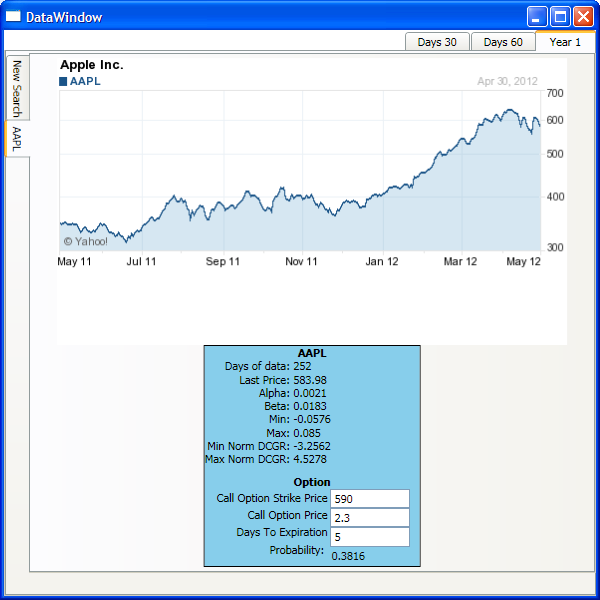
\includegraphics[scale=.6]{screenshot.png}
\end{center}
\end{document}